\documentclass[../TDM1-M2.tex]{subfiles}%

\begin{document}
\section[s]"2"{Plan incliné et frottements solides}

\enonce{%
	\noindent
	\begin{isd}[righthand ratio=.4]
		On considère un plan incliné d'un angle $\alpha = \ang{20;;}$ par rapport à
		l'horizontale. Une brique de masse $m = \SI{600}{g}$ est lancée depuis le
		bas du plan vers le haut, avec une vitesse $v_0 = \SI{2.4}{m.s^{-1}}$. Pour
		étudier le mouvement, on utilise le repère (O,$x$,$y$) avec O coïncidant
		avec la position de départ de la brique. On note $g$ l'accélération de la
		pesanteur, avec $g = \SI{9.81}{m.s^{-2}}$.
		\tcblower
		\begin{center}
			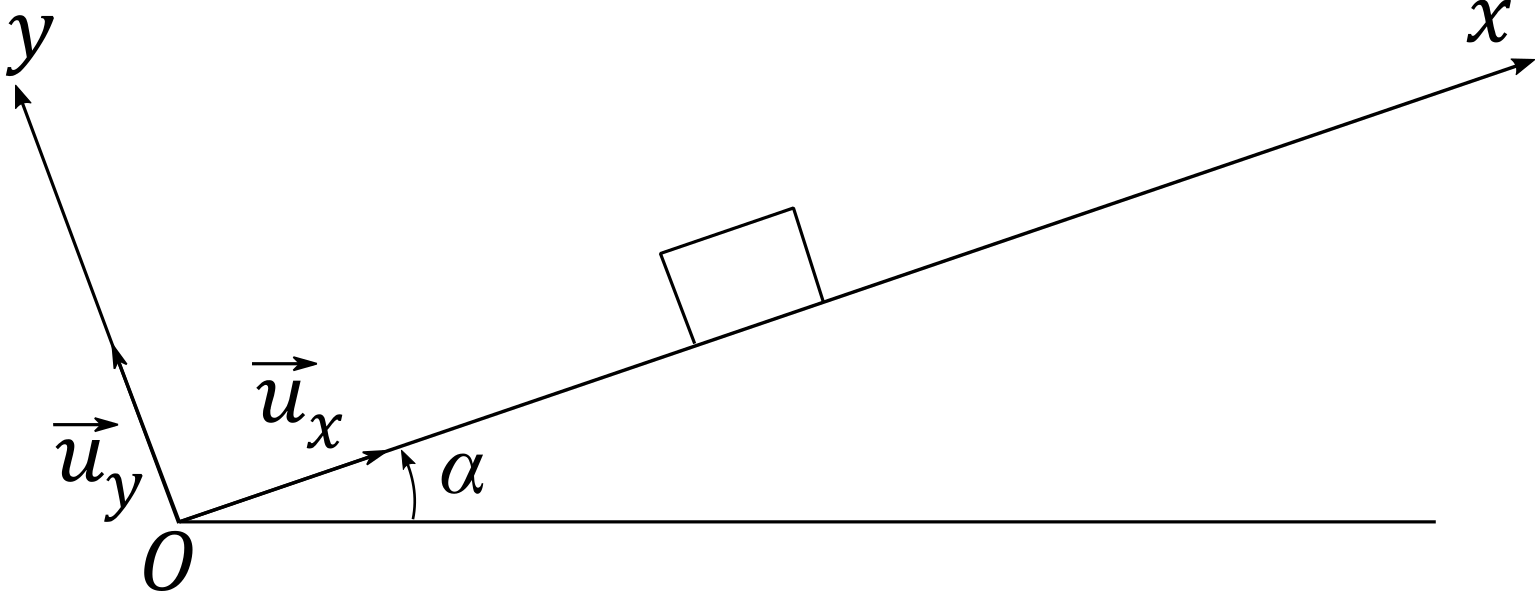
\includegraphics[width=\linewidth]{plan_incl-plain}
		\end{center}
		\vspace{-25pt}
	\end{isd}
}

\begin{blocQR}
	\item On suppose en premier lieu que le contact entre la brique et le plan
	incliné se fait sans frottements
	\resetQ
	\QR{%
		Établir l'équation horaire du mouvement de la brique lors de
		sa montée.
	}{%
		~
		\vspace{-15pt}
		\smallbreak
		\begin{itemize}
			\item[b]{Système}~: \{brique\}
			\item[b]{Référentiel}~: galiléen $(\Or, \ux, \uy)$ (voir schéma)
			\item[b]{Repérage}~: $\OM(t) = x(t)\ux + y(t)\uy$, $\vf(t) = \xp(t)\ux +
				      \yp(t)\uy$, $\af(t) = \xpp(t)\ux + \ypp(t)\uy$
			\item[b]{O et $t$ initial}~: tels que $\OM(0) = \of$
			\item[b]{Vitesse initiale}~: $\vf(0) = v_0\ux$
			\item[b]{Bilan des forces}~:
			      \[
				      \begin{array}{ll}
					      \textbf{Poids}    & \Pf = -mg\cos\a\uy - mg\sin\a\ux \\
					      \textbf{Réaction} & \Rf = R\uy
				      \end{array}
			      \]
			\item[b]{PFD}~:
			      \begin{gather*}
				      m\af = \Pf + \Rf
				      \Lra
				      \left\{
				      \begin{array}{rcl}
					      \cancel{m}\xpp & = & -\cancel{m}g\sin\a \\
					      \underbrace{\cancel{m\ypp}}_{=0}
					                     & = & -mg\cos\a + R
				      \end{array}
				      \right.
			      \end{gather*}
		\end{itemize}
		Il n'y a pas de mouvement sur $\uy$ étant donné que le mouvement
		se fait selon $\ux$~; ainsi $\boxed{y = \yp = \ypp = 0}$, et la
		seconde équation donne
		\[R = mg\cos\a\]
		On intègre la première pour avoir l'équation horaire sur $x(t)$~:
		\begin{gather*}
			\xp(t) = -gt\sin\a+v_0
			\Ra
			\boxed{x(t) = -\frac{1}{2}gt^2\sin\a + v_0t}
		\end{gather*}
		avec les conditions initiales $\xp(0) = v_0$ et $x(0) = 0$.
	}

	\QR{%
		Déterminer la date à laquelle la brique s'arrête, ainsi que la
		distance qu'elle aura parcourue.
	}{%
		On trouve le temps d'arrêt quand la vitesse est nulle. Soit
		$t_s$ ce temps d'arrêt~:
		\begin{gather*}
			\xp(t_s) = 0
			\Lra
			v_0 = gt_s\sin\a
			\Lra
			\boxed{t_s = \frac{v_0}{g\sin\a}}
		\end{gather*}
		On remarque alors que si $\a = 0$, $t_s \rightarrow +\infty$, ce
		qui est logique puisque sans frottement la brique ne
		s'arrêterait jamais. On obtient la distance d'arrêt en injectant
		ce temps dans $x(t)$~:
		\begin{gather*}
			x(t_s) = -\frac{1}{2}\cancel{g}
			\frac{v_0{}^2}{g^{\cancel{2}}\sin^{\bcancel{2}}\a}
			\bcancel{\sin\a} + v_0 \frac{v_0}{g\sin\a}
			\Lra
			\boxed{x(t_s) = \frac{1}{2}\frac{v_0{}^2}{g\sin\a}}
		\end{gather*}
	}

	\item On suppose ensuite qu'il existe des frottements solides, avec $f$ le
	coefficient de frottements solides tel que $f = \num{0.20}$.
	\resetQ
	\QR{%
		Établir l'équation horaire du mouvement de la brique lors de
		sa montée.
	}{%
		On reprend le même système, mais le bilan des forces change~:
		\begin{itemize}
			\item[b]{Bilan des forces}~:
			      \[
				      \begin{array}{ll}
					      \textbf{Poids}    & \Pf = -mg\cos\a\uy - mg\sin\a\ux \\
					      \textbf{Réaction} & \Rf = R_N\uy -R_T\ux
				      \end{array}
			      \]
			      En effet, sur la montée de la brique, sa vitesse est
			      dirigée vers $+\ux$, donc la force de frottement (qui
			      est une force de freinage et donc opposée à la vitesse)
			      est dirigée vers $-\ux$. De plus, avec les lois du
			      frottement de \textsc{Coulomb}, sur la montée la brique
			      glisse sur le support, on a donc
			      \[\boxed{R_T = fR_N}\]
			\item[b]{PFD}~:
			      \begin{gather*}
				      m\af = \Pf + \Rf
				      \Lra
				      \left\{
				      \begin{array}{rcl}
					      m\xpp & = & -mg\sin\a - fR_N \\
					      \underbrace{\cancel{m\ypp}}_{=0}
					            & = & -mg\cos\a + R_N
				      \end{array}
				      \right.
			      \end{gather*}
		\end{itemize}
		Il n'y a pas de mouvement sur $\uy$ étant donné que le mouvement
		se fait selon $\ux$~; ainsi $\boxed{y = \yp = \ypp = 0}$, et la
		seconde équation donne
		\[R_N = mg\cos\a\]
		Que l'on réinjecte dans la première~:
		\[\xpp = -g\sin\a - fg\cos\a\]
		On intègre cette dernière pour avoir l'équation horaire sur $x(t)$~:
		\begin{gather*}
			\xp(t) = -g(\sin\a + f\cos\a)t+v_0
			\Ra
			\boxed{x(t) = -\frac{1}{2}g(\sin\a + f\cos\a)t^2 + v_0t}
		\end{gather*}
		avec les conditions initiales $\xp(0) = v_0$ et $x(0) = 0$. On
		retrouve le résultat précédent en posant $f=0$.
	}

	\QR{%
		Déterminer la date à laquelle la brique s'arrête, ainsi que la
		distance qu'elle aura parcourue.
	}{%
		On trouve le temps d'arrêt quand la vitesse est nulle. Soit
		$t_s$ ce temps d'arrêt~:
		\begin{gather*}
			\xp(t_s) = 0
			\Lra
			v_0 = gt_s(\sin\a + f\cos\a)
			\Lra
			\boxed{t_s = \frac{v_0}{g(\sin\a + f\cos\a)}}
		\end{gather*}
		Ce temps est plus \textbf{court} que sans frottements. On
		obtient la distance d'arrêt en injectant ce temps dans $x(t)$~:
		\begin{gather*}
			x(t_s) = -\frac{1}{2}\cancel{g(\sin\a + f\cos\a)}
			\frac{v_0{}^2}{\left(g(\sin\a + f\cos\a)\right)^{\cancel{2}}}
			+ v_0 \frac{v_0}{g(\sin\a + f\cos\a)}\\
			\Lra
			\boxed{x(t_s) = \frac{1}{2}\frac{v_0{}^2}{g(\sin\a + f\cos\a)}}
		\end{gather*}
	}

	\item On suppose finalement que la brique est \textbf{posée} sur le plan
	avec $\alpha$ variable.
	\resetQ
	\QR{%
		Quel doit être l'angle $\alpha$ pour que l'objet se mette en
		mouvement~?
	}{%
		Cette fois, la brique est initialement à l'arrêt, soit $\af(0)
			= \of$, et la brique ne glisse pas donc $R_T < fR_N$. On aura
		mouvement quand il y aura glissement, c'est-à-dire quand $R_T =
			fR_N$. On reprend donc le système précédent avec $\af = \of$~:
		\begin{gather*}
			\underbrace{\bcancel{m\af}}_{=\of} = \Pf + \Rf
			\Lra
			\left\{
			\begin{array}{rcl}
				0 & = & -mg\sin\a - fR_N \\
				0 & = & -mg\cos\a + R_N
			\end{array}
			\right.
			\Lra
			\left\{
			\begin{array}{rcl}
				\sin\a & = & f\cos\a  \\
				R_N    & = & mg\cos\a
			\end{array}
			\right.\\
			\Lra
			f = \tan\a
			\Lra
			\boxed{\alpha = \atan(f)}
		\end{gather*}
	}

	\QR{%
		Si le plan est en bois et la brique en métal, donner la valeur
		de cet angle. Même question si la brique est en bois. On donne
		\[
			f_{\text{fer/chêne}} = \num{0.26}
			\qet
			f_{\text{chêne/chêne}} = \num{0.34}
		\]
	}{%
		\leftcenters{On trouve}{
			$\boxed{\a\ind{fer/chêne} = \ang{14}}
				\qet
				\boxed{\a\ind{chêne/chêne} = \ang{19}}
			$}
	}

	\item Avec $\alpha = \ang{0;;}$, on souhaite déplacer une armoire de
	\SI{100}{kg} en tirant dessus avec la force $\Ff$. On donne
	$f_{\text{armoire/sol}} = \num{0.25}$.
	\resetQ
	\QR{%
		Déterminer la valeur de $\Ff$ pour mettre en mouvement
		l'armoire.
	}{%
		\begin{itemize}
			\item[b]{Système}~: \{armoire\}
			\item[b]{Référentiel}~: $(\Or, \ux, \uy)$ avec $\uy$ vertical
			      asendant
			\item[b]{Repère}~: On suppose la force de traction dirigée
			      vers $+\ux$, et donc la vitesse de l'armoire selon $+\ux$
			\item[b]{Repérage}~: $\OM = x(t)\ux$, $\vf = \xp(t)\ux$, $\af = \xpp(t)\ux$
			\item[b]{Bilan des forces}~:
			      \[
				      \begin{array}{ll}
					      \textbf{Poids}                 & \Pf = m\gf = -mg\uy \\
					      \textbf{Réaction normale}      & \Rf_N = R_N\uy      \\
					      \textbf{Réaction tangentielle} & \Rf_T =
					      -R_T\ux                                              \\
					      \textbf{Traction}              & \Ff = F\ux
				      \end{array}
			      \]
			      À la limite du glissement, on a $R_T = fR_N$.
			\item[b]{PDF}~: quand le mouvement est lancé, l'accélération est
			      nulle.
			      \begin{gather*}
				      \underbrace{\bcancel{m\af}}_{=0}
				      = \Pf + \Rf_N + \Rf_T + \Ff
				      \Lra
				      \left\{
				      \begin{array}{rcl}
					      0 & = & -mg + R_N \\
					      0 & = & F - fR_N
				      \end{array}
				      \right.\\
				      \Lra
				      \left\{
				      \begin{aligned}
					      R_N       & = mg   \\
					      \Aboxed{F & = fmg}
				      \end{aligned}
				      \right.
				      \qavec
				      \left\{
				      \begin{array}{rcl}
					      m & = & \SI{100}{kg}      \\
					      g & = & \SI{10}{m.s^{-2}} \\
					      f & = & \num{0.25}
				      \end{array}
				      \right.\\
				      \AN
				      \boxed{F = \SI{250}{N}}
				      \Lra
				      \boxed{\frac{F}{g} = \SI{25}{kg}}
			      \end{gather*}
		\end{itemize}
		Ainsi, il suffit de fournir une force égale à un quart du poids.
	}

	\QR{%
		En déduire à quoi sert de mettre des patins en téflon sur les
		pieds de l'armoire.
	}{%
		Mettre des patins permet de diminuer le coefficient de
		frottement, et donc de diminuer la force de traction nécessaire
		pour déplacer le meuble.
	}
\end{blocQR}

% La réaction $\Rf$ du plan sur la brique s'exprime donc $\Rf = \Nf + \Tf$, avec
% $\Tf$ colinéaire de sens contraire au vecteur vitesse
\end{document}
